\documentclass{article}

\usepackage[svgnames]{xcolor}

\usepackage[margin=1in]{geometry}
\usepackage{amsmath, amssymb, amsthm}
\usepackage{enumitem}

%Subfigures
\usepackage{subcaption}

%Links
\usepackage[colorlinks]{hyperref}

%Drawing Graphs
\usepackage{tikz}
\usepackage{pgfplots} \pgfplotsset{compat=1.15} 
\usepackage{ifthen}
    %Arrows on curve, don't understand how it works
    \usetikzlibrary{arrows.meta,positioning}
    \usetikzlibrary{decorations.markings}
    \tikzset{
        set arrow inside/.code={\pgfqkeys{/tikz/arrow inside}{#1}},
        set arrow inside={end/.initial=>, opt/.initial=},
        /pgf/decoration/Mark/.style={
            mark/.expanded=at position #1 with
            {
                \noexpand\arrow[\pgfkeysvalueof{/tikz/arrow inside/opt}]{\pgfkeysvalueof{/tikz/arrow inside/end}}
            }
        },
        arrow inside/.style 2 args={set arrow inside={#1},
        postaction={
                decorate,decoration={
                    markings,Mark/.list={#2}
                }
            }
        },
    }


%Fancy Footnotes
\newcommand{\fancyfootnotetext}[2]{
  \fancypagestyle{dingens}{\fancyfoot[LO]{\parbox{6cm}{\footnotemark[#1]\footnotesize #2}}}\thispagestyle{dingens}
 }
 
%Cases Environment
\newlist{Cases}{enumerate}{3}
\setlist[Cases]{leftmargin = .25in, label = {Case \arabic*.}, topsep = 0.01in, itemsep = 0.04in, itemindent = .5in, parsep = 0in}

%Formatting and Spacing
\setitemize[1]{noitemsep, parsep = 5pt, topsep = 5pt}
\setenumerate[1]{label = (\alph*), parsep = 1pt, topsep = 5pt}
\setlength\parindent{0pt}
\linespread{1.15}

%Custom Title Fields
\newcommand{\lectTitle}{Lecture 4 Notes}
\newcommand{\lectTime}{January 24, 2022}
\newcommand{\lectClass}{Honors Discrete Mathematics}
\newcommand{\lectClassInstructor}{Professor Gerandy Brito}
\newcommand{\lectSection}{Spring 2022}
\newcommand{\lectAuthorName}{Sarthak Mohanty}

%Headers and Footers
\usepackage{fancyhdr}
\usepackage{extramarks}
\pagestyle{fancy}
\lhead{\lectTime}
\chead{\lectClass \ (\lectClassInstructor)}
\rhead{\lectTitle}
\cfoot{\thepage}
\renewcommand\headrulewidth{0.4pt}
\renewcommand\footrulewidth{0.4pt}

\title{
    \vspace{2in}
    \textbf{\lectClass:\\ \lectTitle}\\
    \vspace{0.1in}\large{\textit{\lectClassInstructor\ \lectSection}}
    \vspace{3in}
    \author{\textbf{\lectAuthorName}}
    \date{}
}

\begin{document}

\maketitle
\pagebreak

\section*{More Proofs}
    \subsubsection*{Example 1}
    We have already proved the statement ``if $n^{2}$ is odd, then $n$ is odd" using a proof by contraposition. Now, prove this statement using a proof by contradiction.
    
    \vspace{1.5mm}
    \textbf{Solution}
    
    \vspace{1.5mm}
    Suppose $n^{2}$ is odd. Now suppose $n$ is even. Then there exists some $k \in \mathbb{N}$ such that $n = 2k$. Then $n^{2} = (2k)^{2} = 4k^{2} = 2(2k^{2})$, so by definition $n^{2}$ is even. This is a contradiction, hence $n$ is odd.
    
    \vspace{1.5mm}
    \textbf{Example 2}
    
    \vspace{1.5mm}
    Recall a natural number $p$ is prime if the only divisors of $p$ are $1$ and $p$ itself; formally, if $(\forall x \in \mathbb{Z})(\forall y \in \mathbb{Z})(d \mid xy = (d \mid x) \lor (d \mid y))$. Prove that there are infinitely many primes.
    
    \vspace{1.5mm}{\small We will use the following facts: 1) If $y \in \mathbb{N}$ and $y \ne 1$, then there exists a prime number $d$ such that $d$ divides $y$. 2) Let $d, x, y \in \mathbb{N}$. If $d$ divides $x$ and $d$ divides $y$, then $d$ divides $y - x$.}

    \vspace{1.5mm}
    \textbf{Solution}
    
    \vspace{1.5mm}
    Suppose there are a finite number of primes. Let $p_1, p_2, \dots p_n$ be all the primes there are. Let $x = p_n!$ and $y = x + 1$.
    
    \begin{Cases}
        \item Suppose $y$ is prime. Since $y > p_{i}$ for all $1 \le i \le n$, $y \ne p_{i}$. Thus, we have found a new prime number, so there are an infinite number of primes.
        \item Suppose $y$ is not prime. Now because $y \in \mathbb{N}$ and $y \ne 1$, there exists a prime number $q$ such that $q \mid y$. Now $q$ must be one of $p_1, p_2, \dots p_n$, so $q \mid x$. Then $q \mid y - x$, so $q \mid 1$. But since $q$ is prime, $q$ does not divide $1$. This is a contradiction, therefore there are an infinite number of primes.
    \end{Cases}
    In either case, we have proved there must be an infinite number of primes.
    
    \vspace{1.5mm}
    \textbf{Example 3}
    
    \vspace{1.5mm}
    Show that $\sqrt{2}$ is irrational.
    
    \vspace{1.5mm}
    \textbf{Solution}
    
    \vspace{1.5mm}
    Suppose $\sqrt{2}$ is rational. Then there exist $a \in \mathbb{Z}$ and $b \in \mathbb{N}$ such that $\sqrt{2} = \frac{a}{b}$ in lowest terms. Squaring both sides, we obtain $2 = \frac{a^{2}}{b^{2}}$, so $2b^{2} = a^{2}$. Now we can say $a^{2}$ divides $2$, and by Example 1, $a \mid 2$. Since $a^{2} \mid 2$, there exists some $k \in \mathbb{N}$ such that $(2k)^{2} = 2b^{2}$, so $b^{2} = 2k^{2}$, so $b^{2}$ divides $2$, so $b \mid 2$. But $\frac{a}{b}$ is in lowest terms. This is a contradiction, therefore $\sqrt{2}$ is irrational.


    %Create drawing of dominoes
    \vspace{1.5mm}
    \textbf{Example 4}
    
    \vspace{1.5mm}
    Consider the $6 \times 6$ chessboards as shown in Figure 1. Suppose we want to tile these boards with dominoes, where a domino is a $2 \times 1$ rectangle, and a tiling is a way to place several dominoes on the board in any orientation so that all of its squares are covered without overlap.
    \begin{enumerate}
        \item Is a tiling of the chessboard in Figure \ref*{fig:1a} possible?
        \item Is it possible to tile the board after the top left corner has been removed, as in Figure \ref*{fig:1b}?
        \item Is it possible to tile the board after the top left and the bottom right corners have been removed, as in Figure \ref*{fig:1c}?
    \end{enumerate}
    
    \begin{figure}[htbp]
        \centering
        \begin{subfigure}{0.3\textwidth}
            \centering
            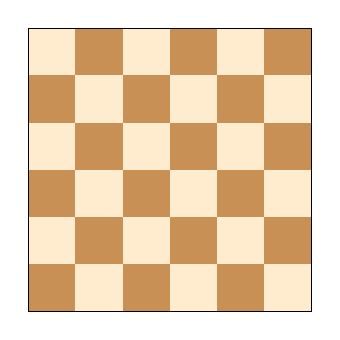
\begin{tikzpicture}[x = 1cm, scale = 0.6]
                \foreach \x in {0,...,5} \foreach \y in {0,...,5}
                {
                    \pgfmathparse{mod(\x+\y,2) ? "BlanchedAlmond" : "BurlyWood!30!brown"}
                    \edef\colour{\pgfmathresult}
                    \path[fill=\colour] (\x,\y) rectangle ++ (1,1);
                }
                \draw (0,0)--(0,6)--(6,6)--(6,0)--cycle;
            \end{tikzpicture}
            \caption{A $6 \times 6$ chessboard.}
            \label{fig:1a}
        \end{subfigure}
        \begin{subfigure}{0.3\textwidth}
            \centering
            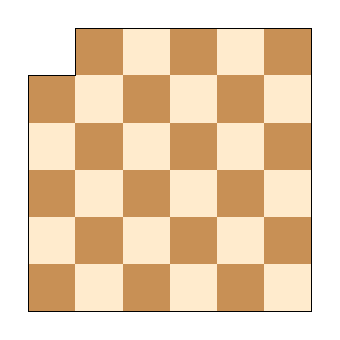
\begin{tikzpicture}[x = 1cm, scale = 0.6]
                \foreach \x in {0,...,5} \foreach \y in {0,...,5}
                {
                    \pgfmathparse{mod(\x+\y,2) ? "BlanchedAlmond" : "BurlyWood!30!brown"}
                    \edef\colour{\pgfmathresult}
                    \path[fill=\colour] (\x,\y) rectangle ++ (1,1);
                }
                \path[fill=White] (0,5) rectangle ++ (1,1);
                \draw (0,0)--(0,5)--(1,5)--(1,6)--(6,6)--(6,0)--cycle;
            \end{tikzpicture}
            \caption{One tile removed.}
            \label{fig:1b}
        \end{subfigure}
        \begin{subfigure}{0.3\textwidth}
            \centering
            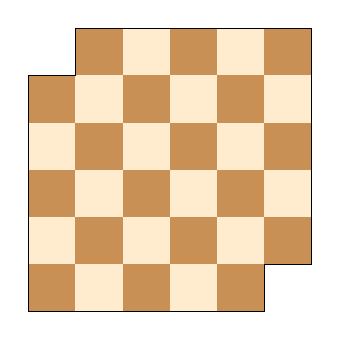
\begin{tikzpicture}[x = 1cm, scale = 0.6]
                \foreach \x in {0,...,5} \foreach \y in {0,...,5}
                {
                    \pgfmathparse{mod(\x+\y,2) ? "BlanchedAlmond" : "BurlyWood!30!brown"}
                    \edef\colour{\pgfmathresult}
                    \path[fill=\colour] (\x,\y) rectangle ++ (1,1);
                }
                \path[fill=White] (0,5) rectangle ++ (1,1);
                \path[fill=White] (5,0) rectangle ++ (1,1);
                \draw (0,0)--(0,5)--(1,5)--(1,6)--(6,6)--(6,1)--(5,1)--(5,0)--cycle;
            \end{tikzpicture}
            \caption{Two tiles removed.}
            \label{fig:1c}
        \end{subfigure}
        \caption{Three chessboard variations.}
        \label{fig:1}
    \end{figure}
    
    \vspace{1.5mm}
    \textbf{Solution}
    \begin{enumerate}
        \item Yes, $18$ dominoes placed vertically will be sufficient.
        \item No, each domino covers an even number of squares, but there are $35$ squares in total, which is odd.
        \item No, note that any domino placed on the chessboard must cover one dark brown and one light brown tile. However, there are $18$ dark brown tiles and only $16$ light brown tiles.
    \end{enumerate}

    \vspace{1.5mm}
    \textbf{Example 5 (Invariants)}
    
    \vspace{1.5mm}
    You are moving on the plane according to the following rule: at every time-step, from $(x, y)$ you go to $(0.6x + 0.8y, 0.8x - 0.6y)$.
    \begin{enumerate}
        \item If you start at the origin can you reach $(1, 1)$?
        \item Can you reach $(1, 1)$ from $(\frac{1}{2}, \frac{1}{2})$? What about any other point $(x, x)$?
    \end{enumerate}
    \vspace{1.5mm}
    \textbf{Solution}
    
    \vspace{1.5mm}
    \begin{enumerate}
        \item No, because $(0, 0)$ maps to itself.
        \item No. There are many ways to think about this. Our solution will follow a recursive approach. Let $r_{t + 1} = \sqrt{x_{t + 1}^{2} + y_{t + 1}^{2}}$ be the distance from the origin to the point at time $t + 1$; in other words, the magnitude of our next location. Then
        \begin{align*}
            r_{t + 1}^{2} &= (0.6x_{t} + 0.8y_{t})^{2} + (0.8x_{t} - 0.6y_{t})^{2} \\
            &= 0.36x_{t}^{2} + 0.64y_{t}^{2} + 0.96x_{t}y_{t} + 0.64x_{t}^{2} + 0.36y_{t}^{2} - 0.96x_{t}y_{t} \\
            &= x_{t}^{2} + y_{t}^{2},
        \end{align*}
        so $r_{t + 1} = \sqrt{x_{t}^{2} + y_{t}^{2}} = r_{t}$. Hence in each time step, we maintain the same radius, as shown in Figure \ref*{fig:2}.
        
        \textbf{TA Remark}: Another way to think about it is (if you have taken Linear Algebra) by expressing the system as a rotation matrix: 
        $$
        \left[\begin{array}{c}
            x_{t + 1} \\
            y_{t + 1}
        \end{array}\right]
        =
        \left[\begin{array}{cc}
            0.6 & -0.8 \\
            0.8 & 0.6
        \end{array}\right]
        \left[\begin{array}{c}
            x_{t} \\
            y_{t}
        \end{array}\right]$$
        Hence after every time-step, we simply rotate the previous location counterclockwise, until eventually we have reached our original point.
        \begin{figure}[htbp]
            \centering
            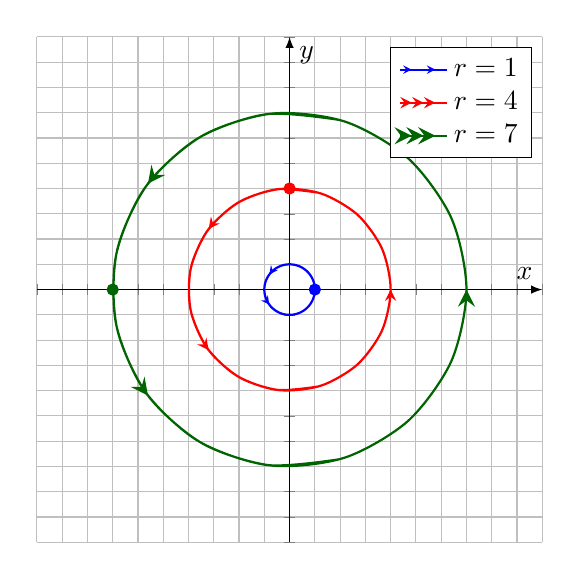
\begin{tikzpicture}
                \begin{axis}[
                    width=8cm, height=8cm,
                    axis lines = center,
                    grid = major,
                    axis line style = -latex,
                    % axis line style = thick,
                    xlabel={$x$}, ylabel={$y$}, 
                    xmin = -10, xmax = 10,
                    ymin = -10, ymax = 10,
                    xtick = {-10,...,10},
                    ytick = {-10,...,10},
                    xticklabels={,,},
                    yticklabels={,,}
                    ]
                    \addplot[samples = 200, blue, thick, arrow inside={end=stealth,opt={blue,scale=.75}}{0.25,0.75}] ({cos(deg(x))}, {sin(deg(x))});
                    \addplot[smooth, red, thick, arrow inside={end=stealth,opt={red,scale=1}}{0.25,0.5,0.75}] ({4*cos(deg(x))}, {4*sin(deg(x))});
                    \addplot[smooth, DarkGreen, thick, arrow inside={end=stealth, opt={DarkGreen,scale = 1.5}}{0.25,0.5,0.75}]  ({7*cos(deg(x))}, {7*sin(deg(x))});
                    \draw[blue, fill] (1,0) circle[radius=2pt];
                    \draw[red, fill] (0,4) circle[radius=2pt];
                    \draw[DarkGreen, fill] (-7,0) circle[radius=2pt];
                    \legend{$r = 1$, $r = 4$, $r = 7$}
                \end{axis}
            \end{tikzpicture}
            \caption{Our path on the plane at different starting points.}
            \label{fig:2}
        \end{figure}
    \end{enumerate}

\section*{Post Lecture}

\subsection*{Question 1}
    There are 100 very small ants at distinct locations on a 1-dimensional meter stick. Each one walks towards one end of the stick, independently chosen, at 1 cm/s. If two ants bump into each other, both immediately reverse direction and start walking the other way at the same speed. If an ant reaches the end of the meter stick, it falls off. Prove that all the ants will always eventually fall off the stick.

\subsection*{Solution(s)}
    Most students find the first solution fairly quickly. However, I added this question as this lecture covered \textit{elegant} proofs, which is more in line with Solution 2.
    
    \vspace{1.5mm}
    \textbf{Solution 1}: If the left-most ant is facing left, it will fall off the left end. Otherwise, it will either fall off the right end or bounce off an ant in the middle and then fall off the left end. So now we have shown at least one ant falls off. But by the same reasoning another ant will fall off, and another, and so on, until they all fall off.
    
    \vspace{1.5mm}
    \textbf{Solution 2}: Now instead, imagine that the ants walk through each other rather than bump off each other. If we view the ants as indistinguishable, this is the same problem, so they all just walk off the meter stick.


\subsection*{Question 2 (Calculus)}
    This question can be solved with the power series taught in Calculus 2.
    \begin{enumerate}
        \item Does there exist an infinite series of irrational numbers whose sum is a rational number?
        \item What about an infinite series of rational numbers whose sum is irrational? 
    \end{enumerate}

\subsection*{Solution}
    \begin{enumerate}
        \item Yes: note that the series $$\sin(x) = \sum_{n = 0}^{\infty} \frac{(-1)^{n}x^{2n + 1}}{(2n + 1)!} = x - \frac{x^{3}}{3!} + \frac{x^{5}}{5!} - \dots$$ converges to a rational number when $x = \pi$.
        \item Again yes: note that the series $$e^{x} = \sum_{n = 0}^{\infty} \frac{x^{n}}{n!} = 0 + x + \frac{x^{2}}{2!} + \frac{x^{3}}{3!} + \dots$$ converges to an irrational number when $x = 1$.
    \end{enumerate}
    In fact, every irrational number can be written as the infinite sum of rational numbers, which is interesting to think about. Unfortunately, the proof of this statement is currently outside the scope of this course; I may return to it when if/when we cover \textit{Cantor's Diagonal Lemma}.

\subsection*{Question 3 (Combinatorics)}
    Prove that $$1 + 2 + \dots + n = \binom{n + 1}{2}.$$
    
    Note: You won't necessarily need the mathematical formula for $\binom{n}{k}$. However, knowing intuitively what ``$n$ choose $k$" represents will be helpful in solving this question. 

\subsection*{Solution(s)}
    \textbf{Solution 1}\footnotemark[1]: 
    
    \fancyfootnotetext{1}{Taken from \href{https://math.stackexchange.com/a/945510/945785}{here}.}
    
    Suppose there are $n + 1$ people in a room. Everyone shakes hands with everyone else (one handshake per pair of people; nobody shakes his or her own hand). Let's count how many handshakes occurred:
    
    \begin{enumerate}[label = \roman*.]
        \item For each pair of people there is one handshake. So there are $\binom{n + 1}{2}$ handshakes.
        \item Line up the people in a row. First person shakes everyone else's hand: $n$ shakes. The next person shakes hands with everyone except the first person: $n - 1$ new shakes. The next person shakes hands with everyone except the first two people: $n - 2$ new shakes. And so on. This gives a total of $n + (n - 1) + (n - 2) + \dots + 1$ handshakes.
    \end{enumerate}
    
    \textbf{Solution 2:} This approach is more visual and relies on Figure 3, shown below. Suppose $n = 6$. Then the yellow circles represent the sum of all numbers from $1$ to $n$. Furthermore, there are $n + 1$ blue circles. The total sum of all unordered pairs of blues circles is equivalent to $\binom{n + 1}{2}$. We can define a mapping of the yellow circles to pairs of blue circles as given in the figure. Note that each yellow circle will be highlighted only once, and the corresponding lines will define a unique pair of blue circles.
    
    \vspace{1.5mm}
    As we will see soon in the coming lectures, if there is such a mapping between two sets, the sets must have the same size. Hence $1 + 2 + \dots + n = \binom{n + 1}{2}$.
    
    \begin{figure}[htbp]
        \centering
        \begin{subfigure}{0.3\textwidth}
            \centering
            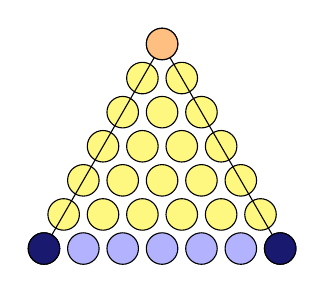
\begin{tikzpicture}[xscale=0.5,yscale=0.5, 
            every node/.style={circle, minimum size = 4mm, inner sep=0pt, outer sep=0pt}]
                \foreach \x in {0,...,6}{
                    \foreach \y in {0,...,\x}{
                        \ifthenelse{\y=0}{
                        \node[draw=black, fill=blue!30] (P-\x-\y) at (\x - \y/2, \y * 0.866) {};
                        }{
                        \node[draw=black, fill=yellow!50] (P-\x-\y) at (\x - \y/2, \y * 0.866) {};
                        }
                    }
                }
                \draw (P-0-0) -- (P-6-6) {};
                \draw (P-6-6) -- (P-6-0) {};
                \node[draw=black, fill=MidnightBlue] at (P-0-0) {};
                \node[draw=black, fill=MidnightBlue] at (P-6-0) {};
                \node[draw=black, fill=orange!50] at (P-6-6) {};
            \end{tikzpicture}
        \end{subfigure}
        \begin{subfigure}{0.3\textwidth}
            \centering
            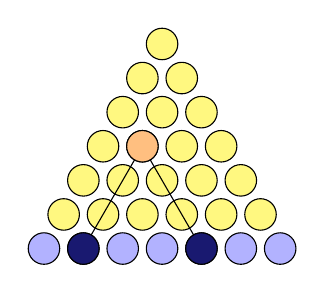
\begin{tikzpicture}[xscale=0.5,yscale=0.5, 
            every node/.style={circle, minimum size = 4mm, inner sep=0pt, outer sep=0pt}]
                \foreach \x in {0,...,6}{
                    \foreach \y in {0,...,\x}{
                        \ifthenelse{\y=0}{
                        \node[draw=black, fill=blue!30] (P-\x-\y) at (\x - \y/2, \y * 0.866) {};
                        }{
                        \node[draw=black, fill=yellow!50] (P-\x-\y) at (\x - \y/2, \y * 0.866) {};
                        }
                    }
                }
                \draw (P-1-0) -- (P-4-3) {};
                \draw (P-4-3) -- (P-4-0) {};
                \node[draw=black, fill=MidnightBlue] at (P-1-0) {};
                \node[draw=black, fill=MidnightBlue] at (P-4-0) {};
                \node[draw=black, fill=orange!50] at (P-4-3) {};
            \end{tikzpicture}
        \end{subfigure}
        \begin{subfigure}{0.3\textwidth}
            \centering
            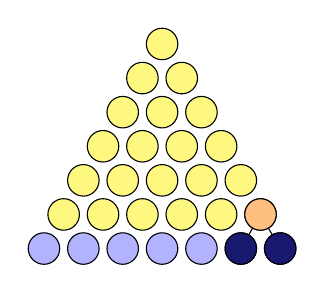
\begin{tikzpicture}[xscale=0.5,yscale=0.5, 
            every node/.style={circle, minimum size = 4mm, inner sep=0pt, outer sep=0pt}]
                \foreach \x in {0,...,6}{
                    \foreach \y in {0,...,\x}{
                        \ifthenelse{\y=0}{
                        \node[draw=black, fill=blue!30] (P-\x-\y) at (\x - \y/2, \y * 0.866) {};
                        }{
                        \node[draw=black, fill=yellow!50] (P-\x-\y) at (\x - \y/2, \y * 0.866) {};
                        }
                    }
                }
                \draw (P-5-0) -- (P-6-1) {};
                \draw (P-6-1) -- (P-6-0) {};
                \node[draw=black, fill=MidnightBlue] at (P-5-0) {};
                \node[draw=black, fill=MidnightBlue] at (P-6-0) {};
                \node[draw=black, fill=orange!50] at (P-6-1) {};
            \end{tikzpicture}
        \end{subfigure}
        \caption{The visualization of the proof for $n = 6$}
        \label{fig:my_label}
    \end{figure}

\subsection*{Question 4}
    Fred brings home 100 kg of potatoes, which consists of 99\% water by mass. He then leaves them outside overnight, at which point they consist of 98\% water by mass. What is their new weight?

\subsection*{Solution}
    Perhaps surprisingly, the answer is $50$ kg.
    
    \vspace{1.5mm}
    At first, 99\% of the 100 kg potato was water, meaning 1\% of 100 kg was 1 kg of solid potato.
    
    \vspace{1.5mm}
    When the water evaporated so that the water is 98\% of the total mass, the mass of the solid in the potato did not change. Hence now 2\% of the total mass is the unchanged 1 kg of solid.
    
    \vspace{1.5mm}
    Finally, 1 kg is 2\% of what? The answer, and therefore the new mass of the potatoes, is 50 kg.
    
\end{document}
